\documentclass{standalone}
\usepackage{picture,color}
\usepackage{graphicx}
\graphicspath{{./examples/}}  % replace your subfolder name 
\setlength{\unitlength}{1in}
\renewcommand{\rmdefault}{phv} % Arial
\renewcommand{\sfdefault}{phv} % Arial

\begin{document}
\begin{picture}(6.9, 4.35)(0,-4.35)  % change your canvas size 
% raw data 
 \put(6.5, -1.2){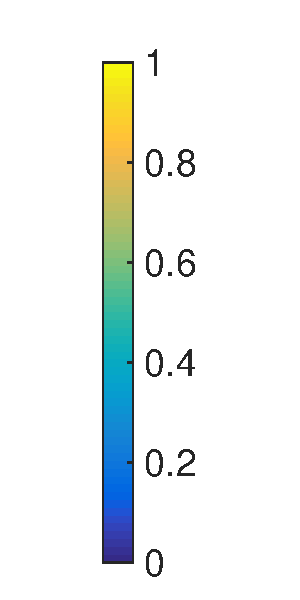
\includegraphics[height=1.15in]{cn_colorbar.pdf}}
\put(0.15, -1.15){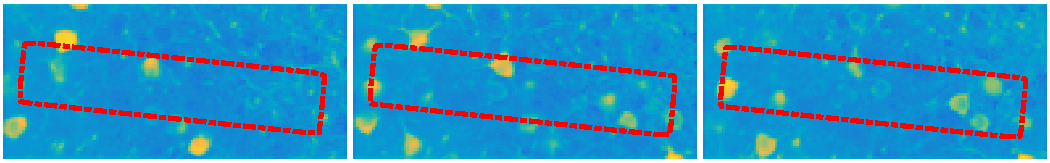
\includegraphics[height=1in]{cn_before.pdf}}
% residual 
\put(0.15, -2.15){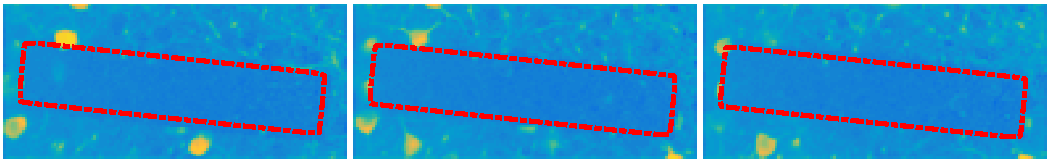
\includegraphics[height=1in]{cn_after.pdf}}
\put(0.05, -1.9){\rotatebox{90}{residual}}
\put(0.01, -0.25){\large\textbf{A}}
\put(0.05, -0.8){\rotatebox{90}{raw}}
\put(5.35, -0.13){slice 3}
\put(3.2, -0.13){slice 2}
\put(1.05, -0.13){slice 1}
% \put(1.1, -0.2){corr. image of the raw data}


% raw data 
\put(6.5, -3.35){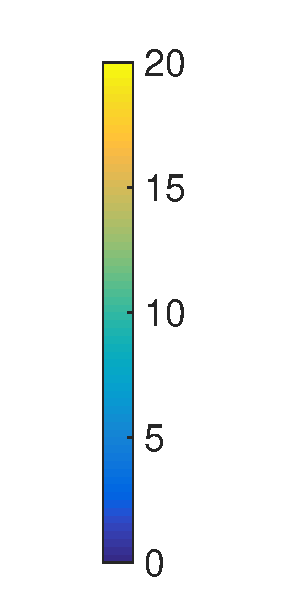
\includegraphics[height=1.15in]{pnr_colorbar.pdf}}
\put(0.15, -3.3){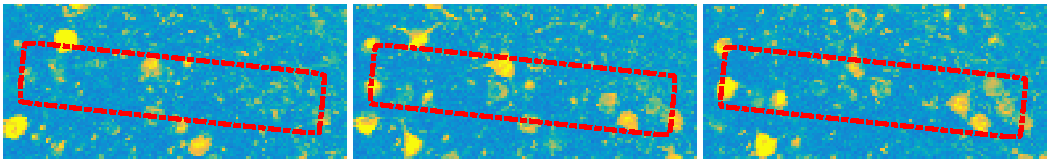
\includegraphics[height=1in]{pnr_before.pdf}}
% residual 
\put(0.15, -4.3){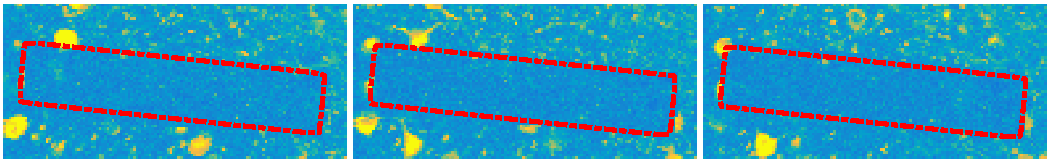
\includegraphics[height=1in]{pnr_after.pdf}}
\put(0.05, -4.05){\rotatebox{90}{residual}}
\put(0.01, -2.4){\large\textbf{B}}
\put(0.05, -2.95){\rotatebox{90}{raw}}
\put(5.35, -0.13){slice 3}
\put(3.2, -0.13){slice 2}
\put(1.05, -0.13){slice 1}

% 
\end{picture}
\end{document}\grid
